\documentclass[conference]{IEEEtran}
\renewcommand{\IEEEkeywordsname}{Keywords}

\usepackage{cite}
\usepackage{amsmath,amssymb,amsfonts}
\usepackage{algorithmic}

% FOOTER
\makeatletter
%%%%%%%%% from https://tex.stackexchange.com/a/200330/161015
\def\ps@IEEEtitlepagestyle{% works only for the first page
    \def\@oddfoot{\customfootnote}%
    \def\@evenfoot{}%
}
\makeatother

\newcommand{\customfootnote}{\hspace{-1.5em}Makalah IF2123 Aljabar Linier dan Geometri -- Teknik Informatika ITB -- Semester I Tahun 2024/2025\hfill}% define /edit here <<<<<<<<<<<<<<<

\usepackage{fancyhdr}
\fancyhf{}
\renewcommand{\headrulewidth}{0pt}
\fancypagestyle{GlobalFootnote}{%
    \lfoot{\customfootnote} 
}
\pagestyle{GlobalFootnote} % style for following pages

\usepackage{graphicx}

\usepackage{textcomp}

\usepackage[hidelinks]{hyperref}
\usepackage{xcolor}

\def\BibTeX{{\rm B\kern-.05em{\sc i\kern-.025em b}\kern-.08em
    T\kern-.1667em\lower.7ex\hbox{E}\kern-.125emX}}
\begin{document}

\title{Implementation of Vector, Linear Transformation, and Quaternion Algebra in the Creation and Manipulation of Bézier Curves for 3D Computer Graphics}

\author{{Z. Nayaka Athadiansyah -- 13523094\textsuperscript{1,2}} \\
\IEEEauthorblockA{\textit{Informatics Engineering Program} \\
\textit{School of Electrical Engineering and Informatics}\\
\textit{Institut Teknologi Bandung, Jl. Ganesha 10 Bandung 40132, Indonesia} \\
\textit{\color{blue} \textsuperscript{1}\href{mailto:13523094@std.stei.itb.ac.id}{13523094@std.stei.itb.ac.id}}, \textit{\color{blue} \textsuperscript{2}\href{mailto:nayaka.zna@gmail.com}{nayaka.zna@gmail.com}}
}
}

\maketitle

\begin{abstract}
Untaian benang takdir mempersatukan kita, Teknik Informatika berjiwa kesatria. Takbir, Allahu Akbar!
\end{abstract}

\begin{IEEEkeywords}
3D computer graphics, bézier curve, linear transformation, quaternion algebra, vector mathematics
\end{IEEEkeywords}

\section{Introduction}Computer graphics has been a broad and rapidly advancing field of research since the 1960s, contributing significantly to innovations across various fields of study\cite{hughes}, such as computer-aided design, virtual reality, and video game development. Computer graphics refers to the science and methods of creating and manipulating visual representations of computer objects\cite{eck}. It also includes the study of visual human-computer interaction, which involves the use of peripheral devices such as visual display units (VDUs) and keyboards to facilitate interaction. It is a multidisciplinary field of research involving engineering, physics, mathematics, computer science, visual art, and behavioral science \cite{hughes}. In this paper, we will limit our discussions to 3D computer graphics exclusively. Hence, whenever we mention "computer graphics," we refer to "3D computer graphics".

\begin{figure}[htb!]
    \centering
    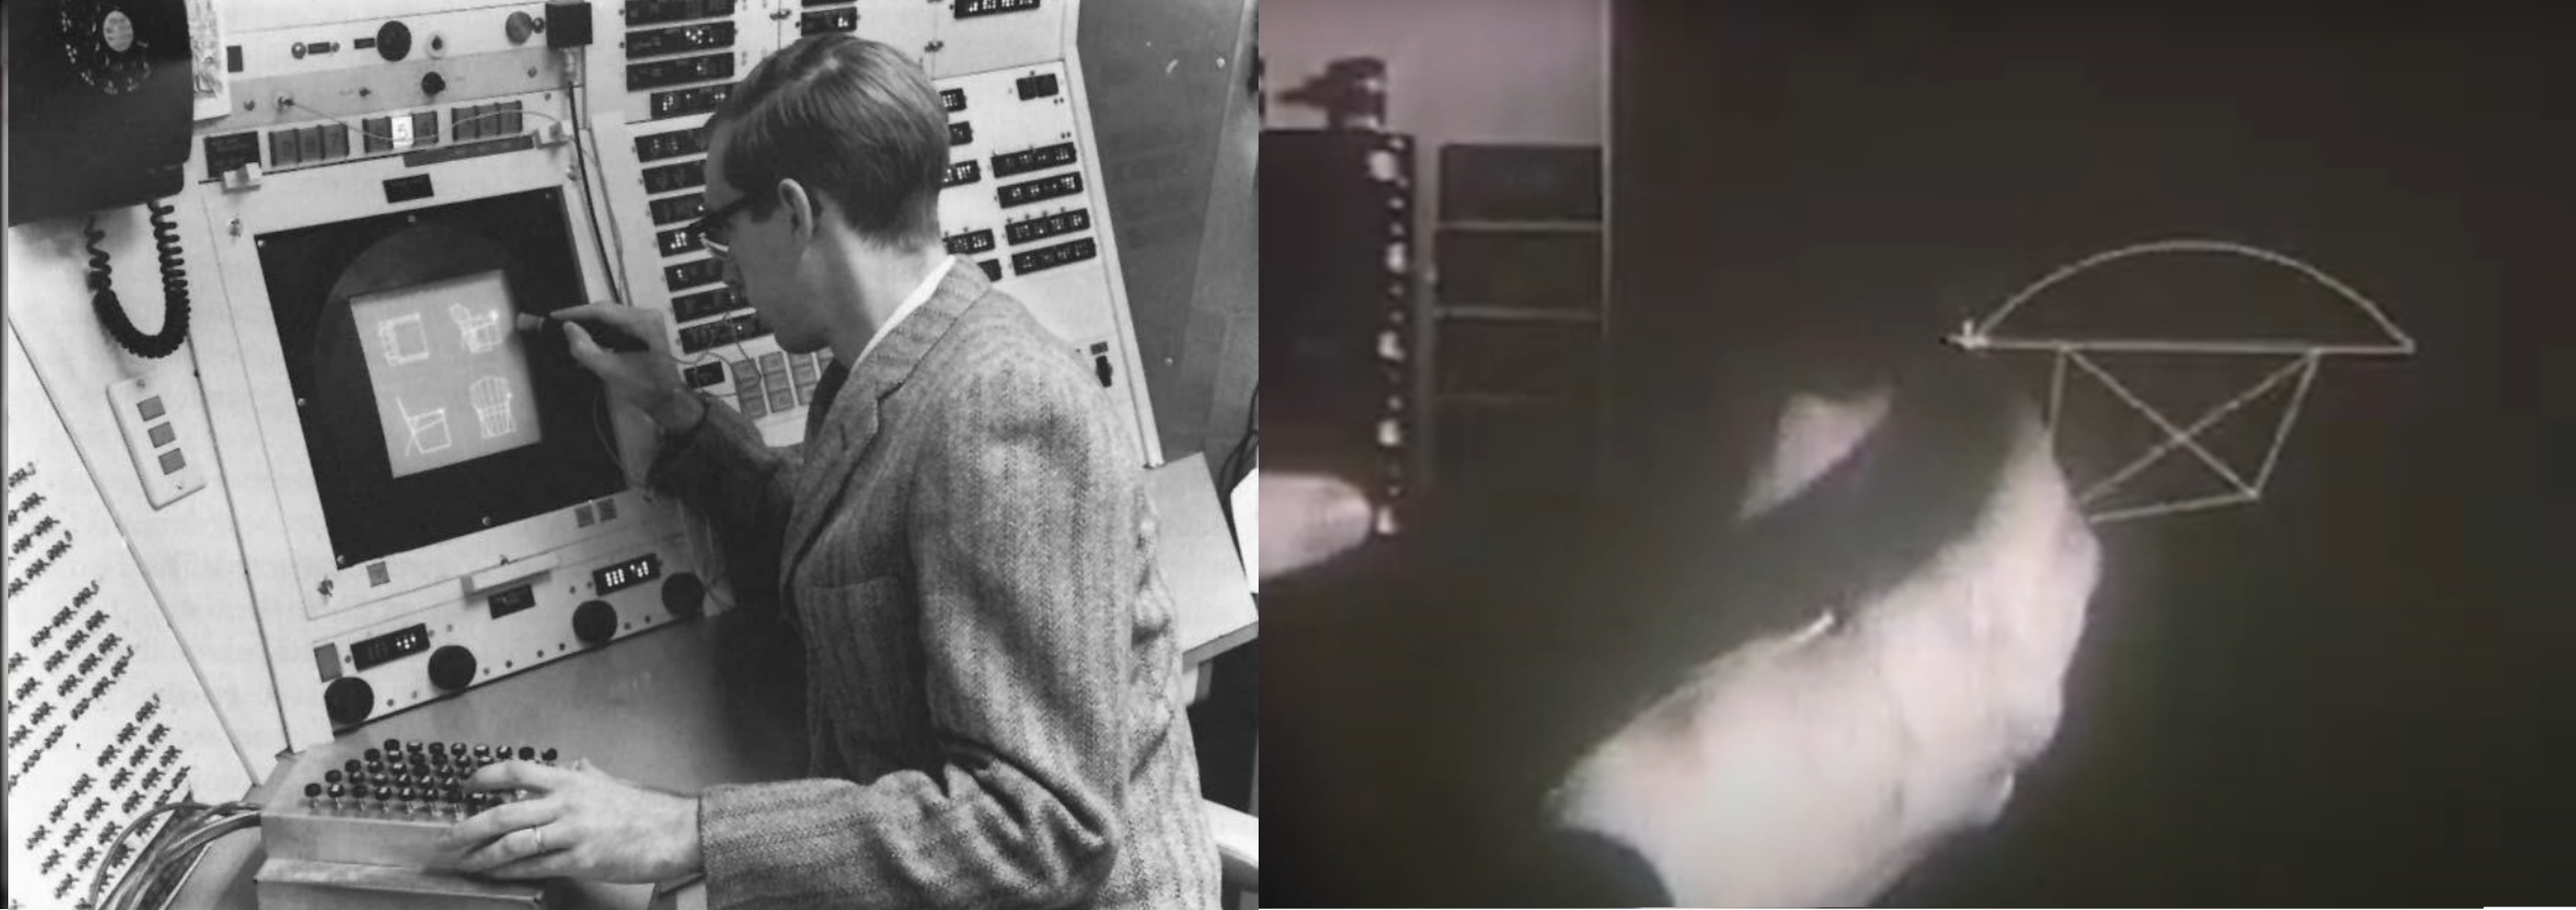
\includegraphics[width=1\linewidth]{sketchpad1.png}
    \caption{A 1963 demonstration of Ivan Sutherland's \textit{Sketchpad}. Source: MIT Lincoln Laboratory}
\end{figure}
In 1963, Ivan Sutherland, an electrical engineering Ph.D. student at MIT Lincoln Laboratory, invented the \textit{Sketchpad}. This innovative computer program marked the beginning of developments in computer graphics\cite{hci}\cite{acm}. \textit{Sketchpad} significantly demonstrated the initial application of a graphical user interface (GUI) and was an early form of computer-aided design (CAD) program, as it was specifically designed to create and interactively modify graphical objects represented as geometrical shapes. The program, written for an MIT Lincoln Laboratory TX-2 computer, involved the usage of a light pen as an input device enabling the creationof geometrical figures using line drawings instead of prompting through keyboard input \cite{sutherland}, making it a real-time interactive GUI program.

\begin{figure}[htb!]
    \centering
    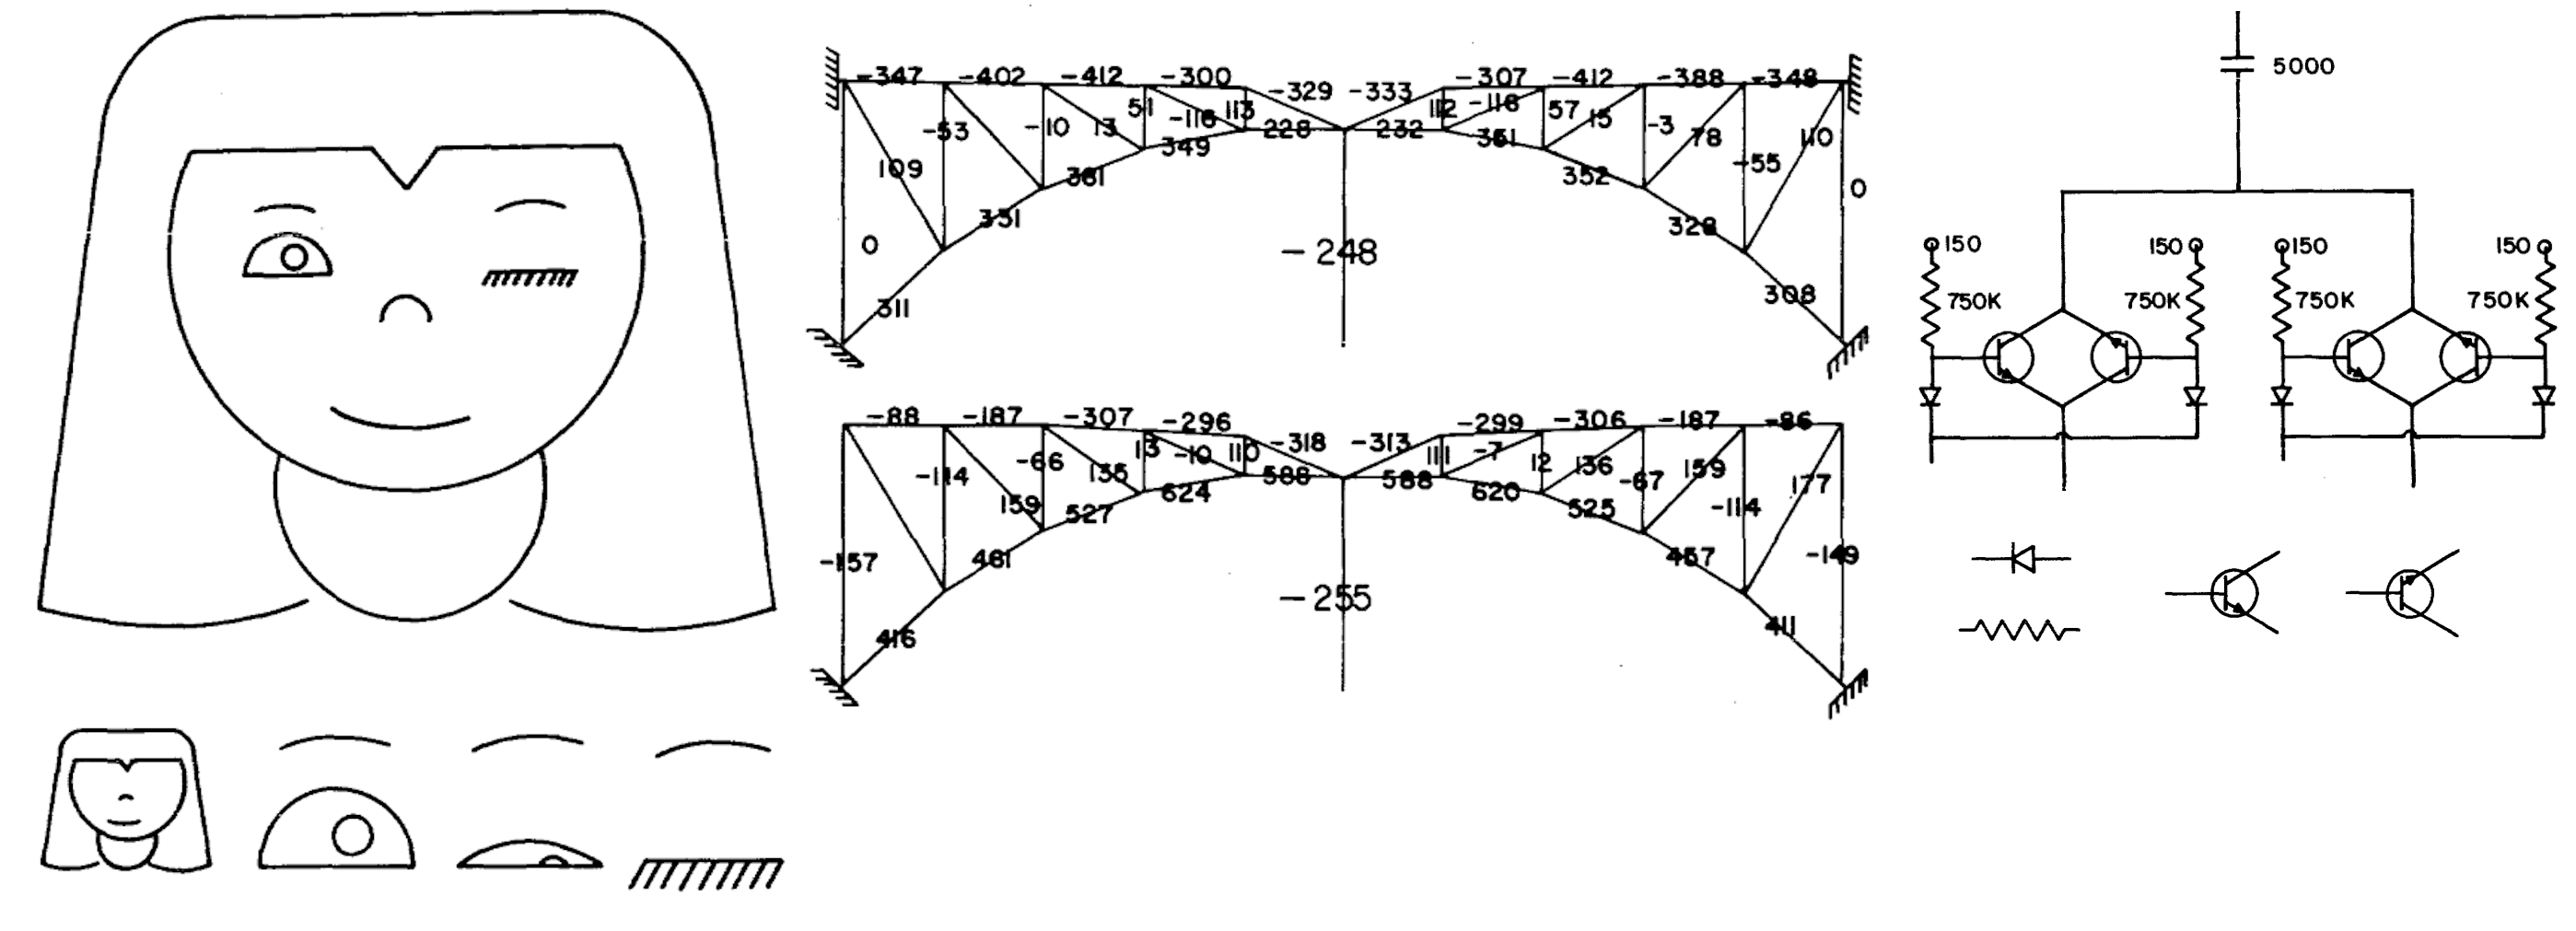
\includegraphics[width=1\linewidth]{sketchpad2.png}
    \caption{Several examples of graphical illustration created in \textit{Sketchpad} (from left): the winking lady 
    "Nefertite" and her graphical component parts; truss diagrams of a cantilever and an arch bridge, with calculations 
    of internal forces in the members; and an electrical circuit. Source: \cite{sutherland}}
\end{figure}
\textit{Sketchpad} users could reuse and combine existing graphical objects to form a new one, letting the users structure its graphical objects hierarchically. Users could also create shapes using constraints. For instance, users could create a parallelogram by constraining the pair of sides to be parallel and having equal length. Sutherland's invention revolutionized human-computer interaction, object-oriented programming, and, especially, computer graphics modeling. Later on, Sutherland and David Evans, a computer science professor from the University of Utah, established Evans and Sutherland to manufacture hardware capable of running computer graphics programs. Due to his innovations, he was awarded the Turing Award in 1988\cite{acm}.


The next decades saw plentiful breakthroughs in the field. Better imagery could be generated due to the development of new methods and algorithms, including Z-buffer algorithm, anti-aliasing, Phong shading, and ray tracing\cite{history}. With a growing enthusiasm for research in computer graphics the Special Interest Group on Computer Graphics and Interactive Techniques (SIGGRAPH) was founded in 1974 as a platform for experts in computer graphics\cite{siggraph}. In the 1980s and 1990s, milestones in computer graphics included the release of 3D computer-animated films such as "Tron," "Toy Story," and "Jurassic Park"; the introduction of 3D modeling software such as Autodesk 3Ds Max and Maya and frameworks such as OpenGL and Direct3D; and the emergence of graphical processing units (GPUs) from companies like NVIDIA\cite{history}\cite{cgi-movie}. These advancements laid the foundations for cutting-edge technologies in the field used today that can be seen everywhere, from entertainment, engineering, medical science, and many electronic appliances that we use daily.

One of the prominent concepts widely used in computer graphics is the Bézier curve. It was discovered in 1962 by the French engineer Pierre Bézier---hence its name. The mathematical groundwork to create such curve, de Casteljau's algorithm, had been discovered earlier in 1959 by Paul de Casteljau, a French mathematician. Bézier curves are defined by a parametric equation and a set of control points, with two points acting as the both ends of the curve while the rest acts as "weights". It is commonly available in computer graphics software, especially in 3D-modeling software like Blender and vector graphics software such as Adobe Illustrator.

\section{Theoretical Foundation}
\subsection{Vector} 
% \textit{Definition and Properties} \\

% \textit{Vector Algebra} \\

\subsection{Linear Transformation} 
% \textit{Matrix Representation} \\

% \textit{Applications in 3D Graphics} \\

\subsection{Quaternion} 
% \textit{Quaternion Algebra} \\

% \textit{Quaternion vs. Euler Angles} \\

\subsection{Spatial Rotation with Quaternion}
% \textit{Quaternion Rotation Formulas} \\

% \textit{Benefits in 3D Graphics} \\

\subsection{Bézier Curve} 
% \textit{Mathematical Definition} \\

% \textit{Control Points and their Role} \\

% \textit{Applications in 3D Computer Graphics} \\

\section{Analysis}

\section{Conclusion}

\section{Appendix}
    The GitHub repository containing the source code for a simple demonstration, as well as the source of several images in this paper, can be accessed \href{https://github.com/nayakazna}{\color{blue} here}. The repository also includes detailed instructions on how to run the code.

\section{Acknowledgment}

\begin{quote}
    \textit{Untaian benang takdir mempersatukan kita, \\
    Teknik Informatika berjiwa kesatria ...}
\end{quote}

I would like to express my heartfelt gratitude to Allah for blessing me with a life filled with miracles. 
I also extend my sincere thanks to Dr. Rinaldi Munir, S.T., M.T., the lecturer for IF2123 Aljabar 
Linear dan Geometri (Linear and Geometry Algebra) K02 class, for his guidance throughout my first semester 
in the Informatics Engineering program at ITB. Moreover, I present my warmest gratitude to Ayesach Svarosstinez
Adhyatman for inspiring the creation of this paper and for her continuous encouragement and support throughout 
its development. Lastly, thanks to Beyoncé.

% Please number citations consecutively within brackets \cite{b1}. The 
% sentence punctuation follows the bracket \cite{b2}. Refer simply to the reference 
% number, as in \cite{b3}---do not use ``Ref. \cite{b3}'' or ``reference \cite{b3}'' except at 
% the beginning of a sentence: ``Reference \cite{b3} was the first $\ldots$''

% Number footnotes separately in superscripts. Place the actual footnote at 
% the bottom of the column in which it was cited. Do not put footnotes in the 
% abstract or reference list. Use letters for table footnotes.

% Unless there are six authors or more give all authors' names; do not use 
% ``et al.''. Papers that have not been published, even if they have been 
% submitted for publication, should be cited as ``unpublished'' \cite{b4}. Papers 
% that have been accepted for publication should be cited as ``in press'' \cite{b5}. 
% Capitalize only the first word in a paper title, except for proper nouns and 
% element symbols.

% For papers published in translation journals, please give the English 
% citation first, followed by the original foreign-language citation \cite{b6}.

\begin{thebibliography}{00}
\bibitem{hughes} J.F. Hughes, \textit{Computer Graphics: Principles and Practice}, 3\textsuperscript{rd} ed. Reading, MA: Addison-Wesley, 1995, pp. 1--10, 598.
\bibitem{eck} D.J. Eck, \textit{Introduction to Computer Graphics}, v.1.4. Accessed Dec. 28 2024. [Online]. Available: \href{https://math.hws.edu/eck/cs424/downloads/graphicsbook-linked.pdf}{https://math.hws.edu/eck/cs424/downloads/graphicsbook-linked.pdf}
\bibitem{hci} A. Sears and J. A. Jacko, \textit{The Human–Computer Interaction Handbook: Fundamentals, Evolving Technologies and Emerging Applications}, 2nd ed. Boca Raton, FL, USA: CRC Press, 2007, p. 5.
\bibitem{acm}  K. A. Frenkel, "An interview with Ivan Sutherland," \textit{Commun. ACM}, vol. 32, pp. 712-714, 1989.
\bibitem{sutherland} I. E. Sutherland, "Sketchpad: A man-machine graphical communication system," in \textit{Proc. May 21-23, 1963, Spring Joint Computer Conference (AFIPS '63 Spring)}, New York, NY, USA, 1963, pp. 329–346. doi: \href{https://doi.org/10.1145/1461551.1461591}{10.1145/1461551.1461591}.
\bibitem{history} K. Sathyanarayana and G. V. V. Ravi Kumar, "Evolution of Computer Graphics and Its impact on Engineering Product Development" in \textit{2008 Fifth International Conference on Computer Graphics, Imaging and Visualisation}, Penang, Malaysia, 2008, pp. 32-37, doi: \href{https://ieeexplore.ieee.org/stamp/stamp.jsp?tp=&arnumber=4626981}{10.1109/CGIV.2008.67}.
\bibitem{siggraph} D. J. Kasik, M. C. Whitton and C. R. Johnson, "The Big 50: Celebrating 50 ACM SIGGRAPH Conferences" in \textit{IEEE Computer Graphics and Applications}, vol. 43, no. 04, pp. 12-80, July-Aug. 2023, doi: \href{https://doi.ieeecomputersociety.org/10.1109/MCG.2023.3266086}{10.1109/MCG.2023.3266086}.
\bibitem{cgi-movie} Z. Sun, “What Does CGI Digital Technology Bring to the Sustainable Development of Animated Films?” in \textit{Sustainability}, vol. 15, no. 14. MDPI AG, p. 10895, Jul. 11, 2023. doi: \href{https://www.mdpi.com/2071-1050/15/14/10895}{10.3390/su151410895}.
\bibitem{strang} G. Strang, \textit{Introduction to Linear Algebra}, 6\textsuperscript{th} ed. Wellesley, MA: Wellesley-Cambridge Press, 2023.
\bibitem{galier} J. Galier, \textit{Curves and Surfaces In Geometric Modeling: Theory And Algorithms}, 2\textsuperscript{nd} ed. Accessed Dec. 28 2024. [Online]. Available: \href{https://www.cis.upenn.edu/~jean/geomcs-v2.pdf}{https://www.cis.upenn.edu/~jean/geomcs-v2.pdf}.
\bibitem{farin} G. Farin, \textit{Curves and Surfaces for CAGD: A Practical Guide}, 5\textsuperscript{th} ed (The Morgan Kaufmann Series in Computer Graphics). San Francisco, CA, USA: Morgan Kaufmann, 2002. doi: \href{https://www.sciencedirect.com/book/9781558607378/curves-and-surfaces-for-cagd}{10.1016/B978-1-55860-737-8.X5000-5}.
\bibitem{lengyel} E. Lengyel, \textit{Mathematics for 3D Game Programming and Computer Graphics}, 3\textsuperscript{rd} ed. Boston, MA, USA: Cengage Learning, 2011, pp. 317--329. ISBN: 978-1-4354-5886-4.
\end{thebibliography}

% \newpage

\section*{Declaration of Originality}
I hereby declare that the work presented in this paper is entirely my own. It is not a copy, translation, or adaptation of any other author's work, and it does not constitute plagiarism.

\begin{flushright}
    Bandung, December, 28\textsuperscript{th} 2024 \\  
    % \includegraphics[width=0.25\linewidth]{ttd.png}\\ % MY SIGNATURE
    Z. Nayaka Athadiansyah – 13523094
\end{flushright}

\end{document}
